%% Artyom Voronin
%%  __     _ _                   
%% / _| __| (_)  _ __  _ __ ___  
%%| |_ / _` | | | '_ \| '_ ` _ \ 
%%|  _| (_| | | | |_) | | | | | |
%%|_|  \__,_|_| | .__/|_| |_| |_|
%%              |_|              
%% Brno, 2021

\documentclass[class=article, crop=false]{standalone}
\usepackage[subpreambles=true]{standalone}
\usepackage{subcaption}

\usepackage{sectsty}
\usepackage{graphicx}
\graphicspath{{img/}{../img/}{../../img/}}
\usepackage{listings}
\lstset{language=Matlab}
\usepackage{hyperref}
\usepackage{amsmath}
\usepackage{import}
\usepackage{subfiles}
\usepackage[utf8]{inputenc}
\usepackage[english]{babel}

%\usepackage[]{todonotes}
\usepackage{xargs}
\usepackage[pdftex,dvipsnames]{xcolor}  % Coloured text etc.
\usepackage[colorinlistoftodos,prependcaption,textsize=tiny]{todonotes}

%\usepackage[square, numbers]{natbib}
%\bibliographystyle{unsrtnat}
%\usepackage[nottoc]{tocbibind}

%\usepackage{biblatex}
%\addbibresource{./citations.bib} %usage \cite{test}
% Margins
% 
\topmargin=-0.45in
\evensidemargin=0in
\oddsidemargin=0in
\textwidth=6.5in
\textheight=9.0in
\headsep=0.25in

%\title{PM and FDI comparison}
%\author{Artyom Voronin} 
%\date{}

\begin{document}
\tableofcontents

% -----------------------------------------------------------------------------
% 
% -----------------------------------------------------------------------------
\section{Theoretical Survey (10-13 pages)}
Why FDA and PdM are useful? Similarities/Differences?
The relative arrangement PdM and FDI methods representing in following
figure \ref{fig:fdi_pm}
\begin{figure}[h!]
    \centering
    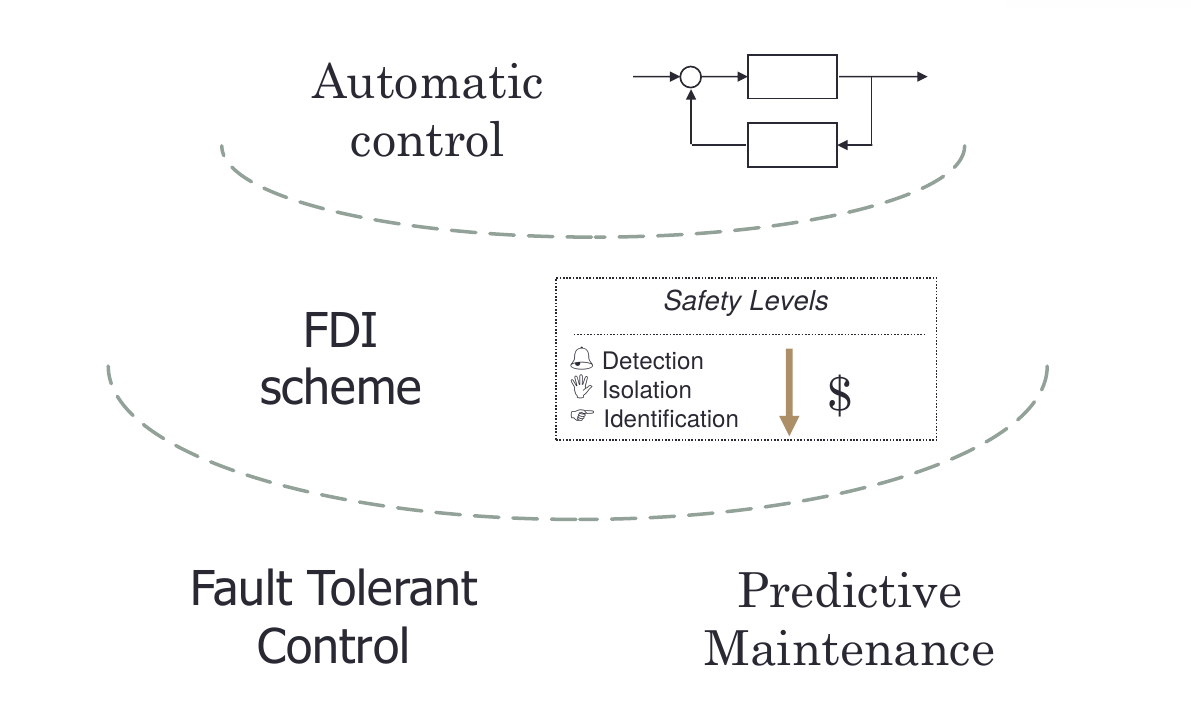
\includegraphics[scale=0.3]{FDI_PM.png}
    \caption{PM and FDI }
    \label{fig:fdi_pm}
\end{figure}



% -----------------------------------------------------------------------------
% 
% -----------------------------------------------------------------------------

\subsection{Problem Definition}

In practice, many types of machinery require some calibration for adequately working,
and online monitoring and classification algorithms can find the problem.

% XXX FaultDetectionMethods-ALiteratureSurvay.pdf


Smart systems = Sensors, but sensors only not doing the system smart. Smart
is combination of sensors, processing signals, extraction useful information and
some decision based on this information.

What kind of sensors to use and which sensor is the best based on
cost/technical efficient perspective.

\begin{itemize}
    \item Fault
    \item Failure   
    \item Malfunction
\end{itemize}

\subsubsection{Types of Faults}
\begin{itemize}
    \item Plant
    \item Sensor
    \item Combination
\end{itemize}

\subsubsection{Types of Maintenance}
\begin{itemize}
    \item{Reactive (fails than fix)}
    \item{Preventative (schedules)}
    \item{Condition-based (based on assess of system)}
    \item{Predictive (based on model that predict failure)}
\end{itemize}






% -----------------------------------------------------------------------------
% 
% -----------------------------------------------------------------------------

\subsection{Fault Detection and Analysis}
Fault Detection and Analysis, FDA. (Fault detection and isolation, FDI) 

\paragraph{FD not new}
FD exists from 60th.

\subsubsection{Goals}

\begin{itemize}
    \item{Fault detection: Detect malfunctions in real time, as soon and as
        surely as possible}
    \item{Fault isolation: Find the root cause, by isolating the system
        components whose operation mode is not nominal}
    \item{Fault identification: Estimation the magnitude (size) and type or
            nature of the fault}
\end{itemize}

%\textbf{Fault \footnotemark detection and isolation} is subfield of control
%engineering, identifying when fault  has occurred, and pinpointing the type
%of fault and its location.

\footnotetext{\textbf{Fault} - not acceptable deviation of at least one characteristic or
parameter of the system from the standard condition.}

\subsubsection{Methods}
Figure \ref{fig:fault_detection} introduce 2 main approaches:

\begin{itemize}
\item{Model-based FDI (compare data with healthy-model)}
\item{Signal processing based FDI (using math methods to extract information
    about the fault from data)}
\end{itemize}

\begin{figure}[h]
    \centering
\begin{subfigure}{0.5\textwidth}
    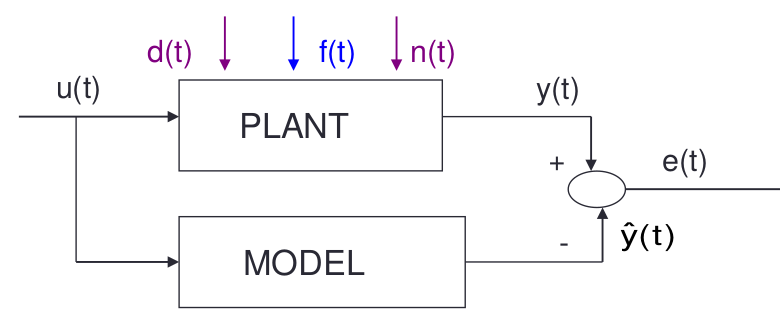
\includegraphics[width=0.9\linewidth]{model_based.png}
    \caption{Model-based fault detection}
    \label{fig:model_based}
\end{subfigure}%
\begin{subfigure}{0.5\textwidth}
    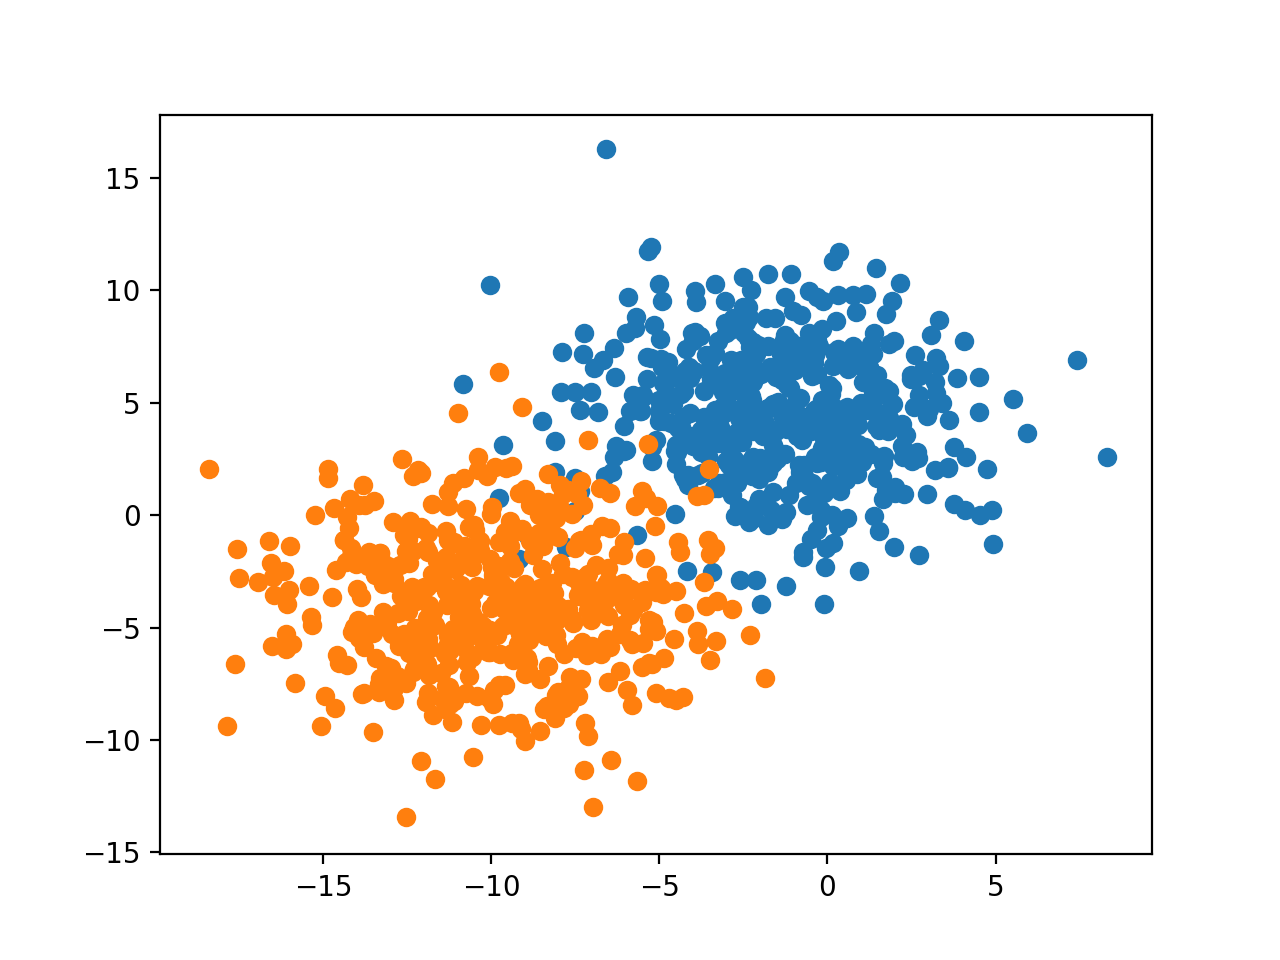
\includegraphics[width=0.9\linewidth]{signal_based.png}
    \caption{Signal-based fault detection}
    \label{fig:signal_based}
\end{subfigure}
\caption{Fault detection common approaches}
\label{fig:fault_detection}
\end{figure}

\paragraph{Signal-Based methods}
\begin{itemize}
    \item Limit Checking and Trend Checking
    \item Data Analysis (PCA)
    \item Spectral Analysis
    \item Parametric Signal Models
    \item Pattern Recognition (kNN, ANN, SOM)
\end{itemize}

\paragraph{Model-Based methods}
We know system structure. Faults modeled as some system variables changes.
Parameter estimation

\paragraph{Knowledge-Based methods}
We know some Expert Knowledge about system behavior. Fuzzy,
confidence-numbers, probability density functions, logic
fault-symptom-tree, if-then rules.

The result of FDI is the detection and identification of faults that occur
during the operation of the device. Subsequently data is processed using
Fault Tolerance and Predictive maintenance methods.

\textbf{Fault Tolerance}: Provide the system with the hardware architecture and
  software mechanisms which will allow, if possible to achieve a given
  objective not only in normal operation, but also in given fault
  situations.


\subsubsection{Condition Monitoring}
Answer to question:"How does system operate now?"
CM gives Diagnostic methods that provides alarm or warning, but not
prognostic forecast about the future behavior (Not RUL).

But collected Condition Monitoring information can give information about
system degradation.


There is a optimization between technical and financial possibilities in a
specific situation.

FMECA (Failure Mode, Effect and Criticality Analysis) \\
FTA (Fault Tree Analysis) \\
RCA (Root Cause Analysis) \\


% -----------------------------------------------------------------------------
% 
% -----------------------------------------------------------------------------


\subsection{Predictive maintenance}
\textbf{Predictive maintenance (PdM)} is cost-effective maintenance strategy that
predicts time to failure and warns of an anticipated location where this
could occur.

\subsubsection{Goals}
The are two main goals of Predictive maintenance, RUL (remaining useful
life) estimation and identification where the future failure can appear, or what is
the reason of decreasing RUL. 
As a result of PdM is RUL representing of number cycles, days, or some time
period before fault occurred. And probability where this fault can appear.

Predict where, when and what is the reason of failure (identify primary
factors).


\textbf{Predictive maintenance development sequence}:
\begin{enumerate}
    \item{Collect data (using sensors, math model)}
    \item{Process data (clean up data)}
    \item{Identify Condition Indicators CI}
        \begin{itemize}
            \item{Signal-based CI}
            \item{Model-based CI}
        \end{itemize}
    \item{Fit model (ML techniques)}
    \item{Deploy monitoring and integrate}
    \item{Dashboard (UI)}
\end{enumerate}


\subsubsection{Methods}
There are couples of signal processing and analyzing methods that used in
both PdM and FDI. For example:

\paragraph{Signal-Based} approach is suitable in situation when we have
measurements from system in different operating conditions. 
But there is a problem that Signal-Based approach enable to classify and
learn patterns observed in training dataset. 


\paragraph{Model-Based} approach is to use physical failure models. This
models do not require a large dataset of failure data. And they can work in
situations never observed before. 


%\begin{itemize}
%    \item Spectral Analysis
%    \item Wavelet Analysis
%    \item Wavelet transform
%    \item FFT
%    \item Short Term Fourier Transform
%    \item Gabor Expansion
%    \item Wigner-Ville distribution
%    \item Correlation
%    \item High resolution spectral analysis
%    \item Waveform Analysis
%    \item Time-Frequency Analysis
%    \item PCA
%    \item Machine Learning techniques:
%        \begin{itemize}
%            \item kNN
%            \item ANN
%        \end{itemize}
%\end{itemize}

\subsubsection{Condition Indicators}
Features in PdM field are called Condition Indicators or CI.
Condition Indicators are features extracted from the signals, representing some
system behavior and hides some information about system processing.

Condition indicators represented by three main domain. There are Time
domain, Frequency domain, Time-Frequency domain Condition Indicators.

\begin{itemize}
    \item Time-domain
    \item Frequency-domain
    \item Time-frequency
\end{itemize}

\subsubsection{Fault Classification}

\subsubsection{Remaining useful life}
RUL goal is remaining time before machine requires maintenance. Not only
predict but provide a confidence bound.

\paragraph{RUL Models}:
% https://www.mathworks.com/company/newsletters/articles/three-ways-to-estimate-remaining-useful-life-for-predictive-maintenance.html

Inputs are condition indicators and models depends on data: 1. Lifetime,
Run-to-failure, known threshold for CI.

\begin{itemize}
    \item Similarity model 
    \item Survival model
    \item Degradation model
\end{itemize}


\subsection{Digital twin}
% https://explore.mathworks.com/digital-twins-for-predictive-maintenance

Digital twin is digital representation of the real life system. Can be
represented as a component, a system of components, or as a system of
system.  

\paragraph{Updating digital twin with incoming data} 

Digital twin can be updated with incoming data from sensors. Fitting model
to new data, digital twin represents the current condition state of the
real world object.

\todo[inline]{Rewrite}
Digital twin can hold historical data about behavior of a system
and can be used for simulation system operation in different conditions,
for designing control and simulate future behavior. (RUL, "What-if")

Digital Twins are helpful in the field of Anomaly Detection and Predictive
Maintenance.

Mathematical model of the real world system can be created using different
approaches. Modeling based on Physical modeling (Simscape) data-driven
modeling where system is represented as a "Black box" or some combination
of this approaches.
Model with estimated parameters uses for simulation system behavior in
different working conditions and with different faults during working
process.

\subsubsection{Using Digital Twin in PdM}

Measured data, Generated data from mathematical model, or Synthetic data
(Combination of measured and generated) can be used for assessment of
Condition Indicators. 

%\subsubsection{Detect and Diagnose Faults}
%Using condition indicators on Test data we can analyze actual system state.
%Designing algorithm is iterative process when you try different
%combinations of condition indicators and different models to evaluate best
%results.

\subsection{Comparison PdM and FDA approaches}

\subsection{Application field}

\end{document}

